% Begin the document and set up the style of the document
\documentclass[a4paper,11pt]{article}

\usepackage{graphicx}
\usepackage{caption}
\usepackage{booktabs}
\usepackage{fullpage}
\usepackage{amsmath}

\usepackage{titlesec} % Used to customize the \section command
\titleformat{\section}{\bf}{}{0em}{}[\titlerule] % Text formatting of sections
\titlespacing*{\section}{0pt}{3pt}{3pt} % Spacing around sections

\usepackage{enumitem}

\newcommand{\indep}{\mathrel{\text{\scalebox{1.07}{$\perp\mkern-10mu\perp$}}}}
\newcommand{\ds}{\displaystyle}
\newcommand{\code}{\texttt}
\newcommand{\HRule}{\rule{\linewidth}{0.5mm}} % Defines a new command for the horizontal lines, change thickness here

\begin{document}

\begin{center}
	\LARGE \textbf{Lab 05 Report}
	\HRule\\
\end{center}

\pagenumbering{arabic}

\noindent \code{Lines in this font represent terminal commands and terminal output.}\\
Lines beginning with \code{\$} are the terminal commands that were run.\\
Lines in this font are the answers to the questions.

\section{EXERCISE 1}
\begin{enumerate}[leftmargin=*]
	\item 
		\begin{enumerate}
			\item Maximum segment size is 67.
			\item When the congestion window size reaches 67, the CWND is reset to 0.
			\item TCP Tahoe resets the CWND to 0 upon any packet loss or timeout event.
			\item After CWND is reset to 0, due to packet loss or timeout, TCP Tahoe returns to slow start, until the slow start threshold is reached. After this threshold has been reached, TCP Tahoe transitions to AIMD for increases. This accounts for the intial exponential increase, followed by linear increase until 68 is reached for CWND.
		\end{enumerate}

		\begin{figure}[!htb]
			\centering
		    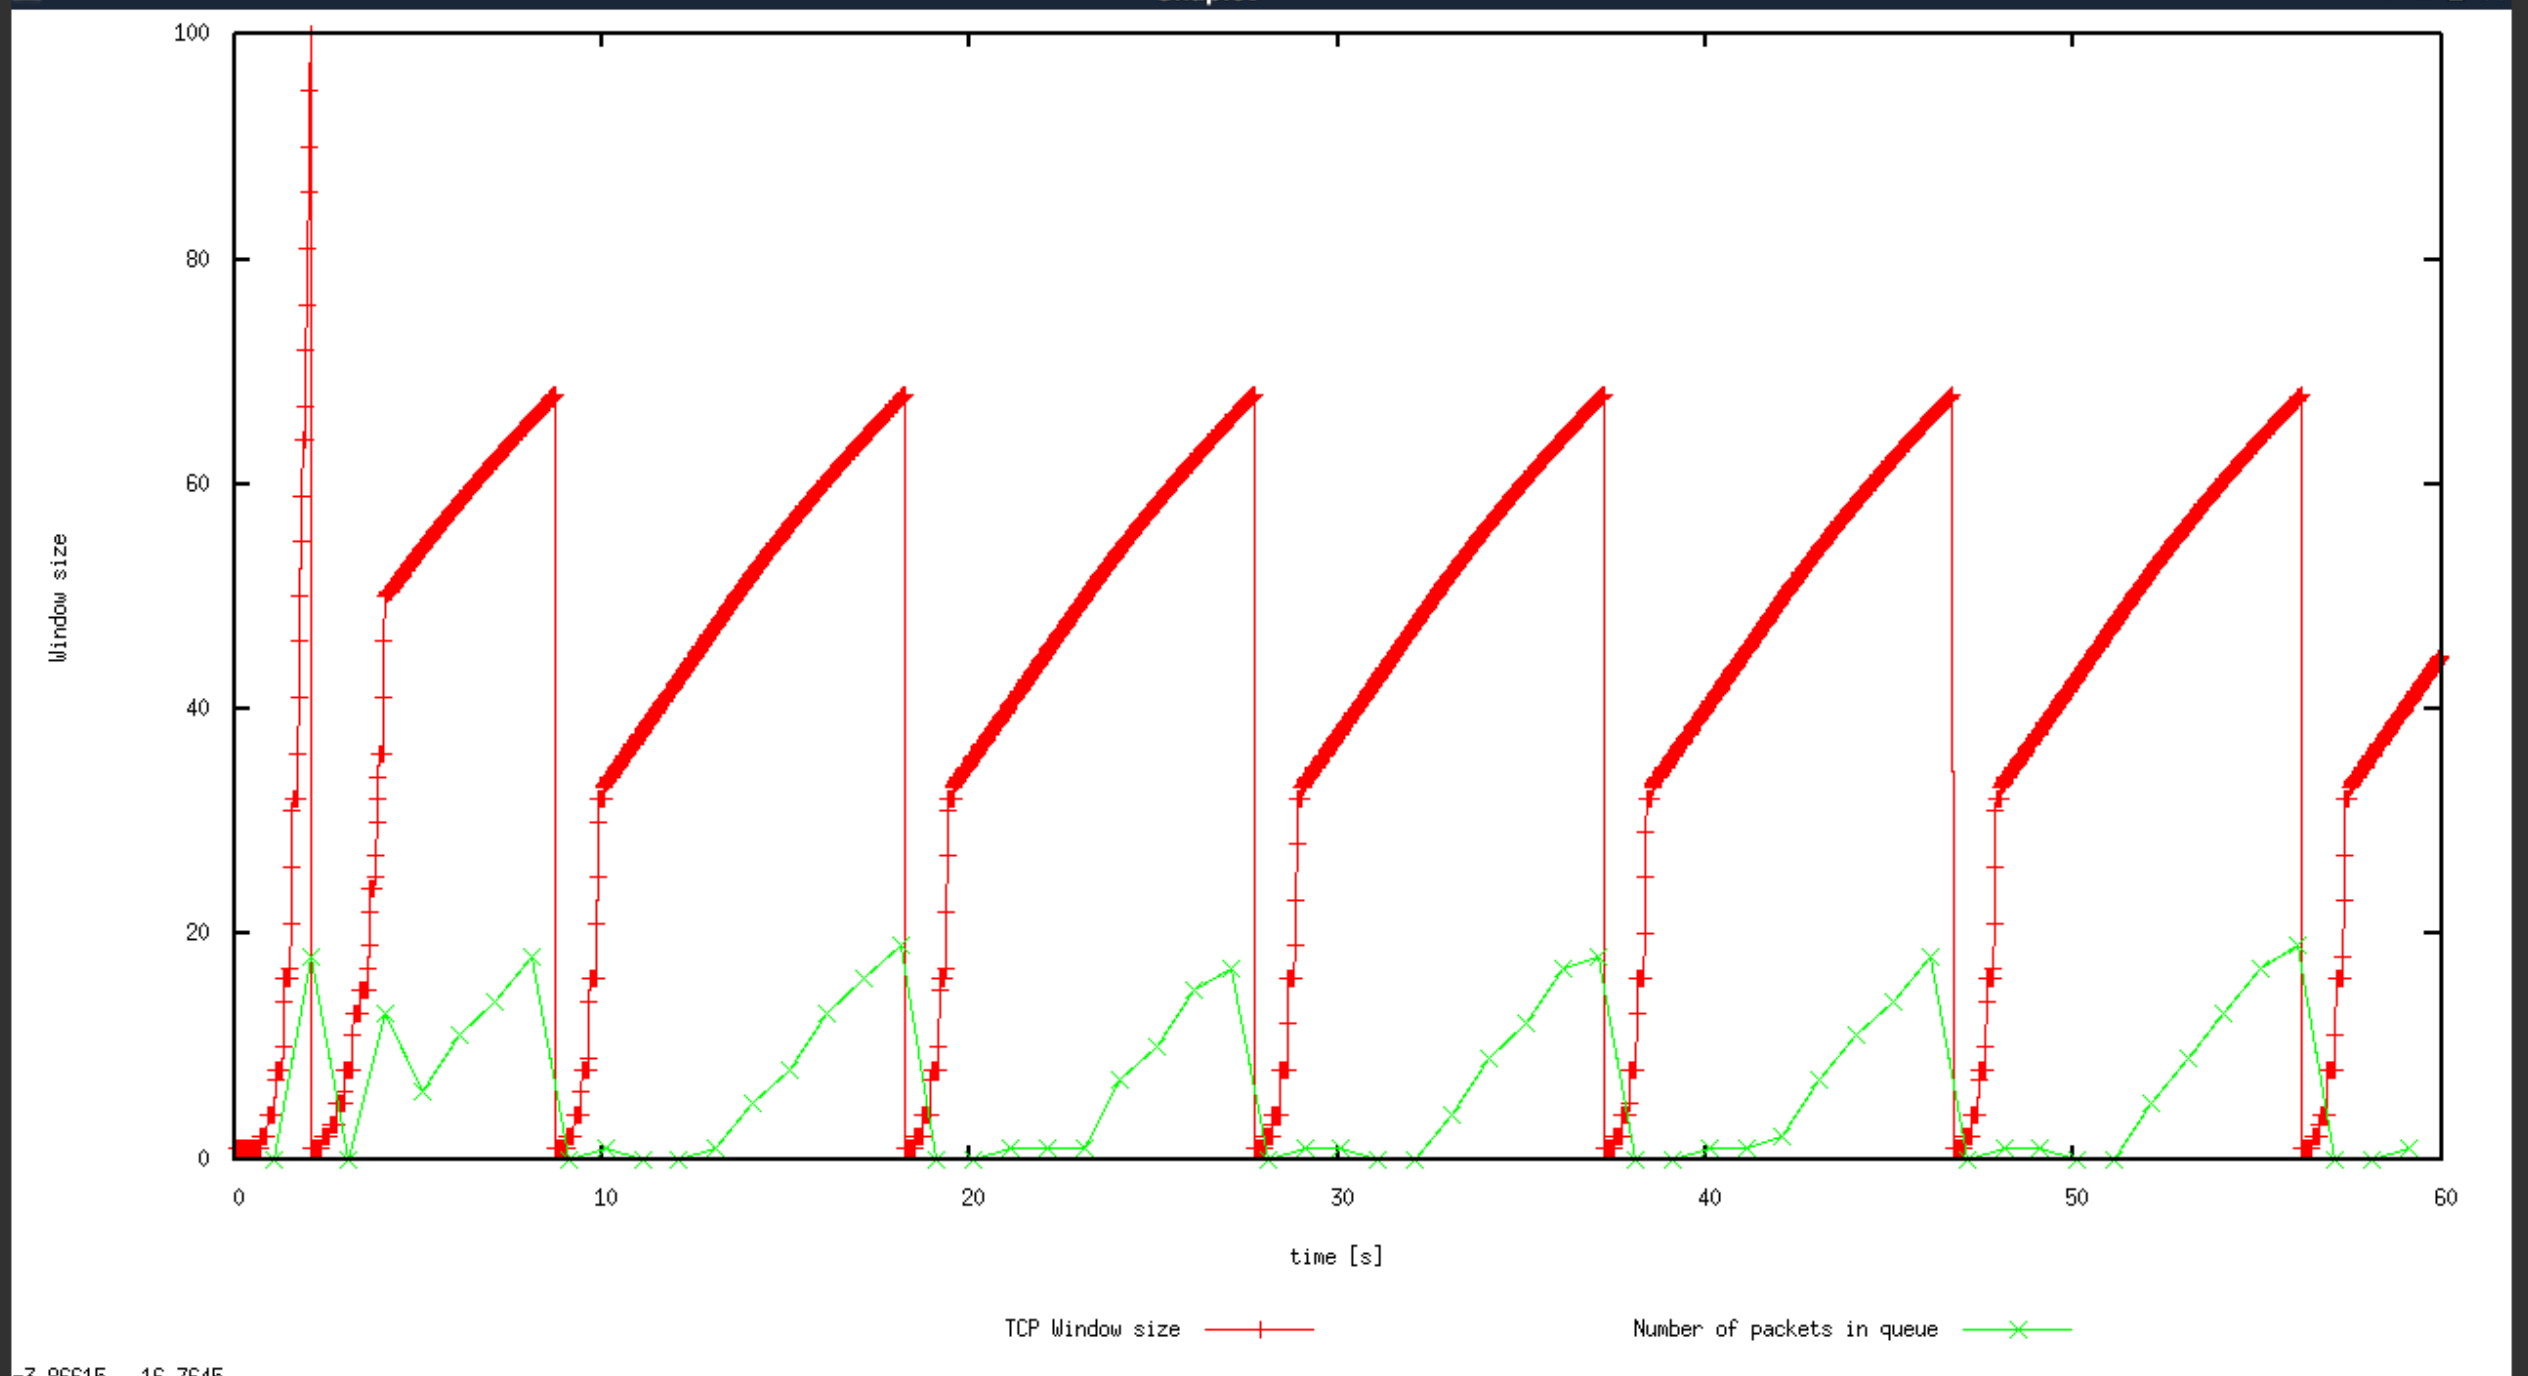
\includegraphics[width=\linewidth, height=0.43\textheight]{tt1f.png}
		\end{figure}

	
	\item Average throughput was 188.976 packets per second. With 540 bytes of data per packet, due to the TCP and IP headers, and 8 bits in a byte, the average throughput becomes 816376.32 bits per second.
		\begin{figure}[!htb]
			\centering
		    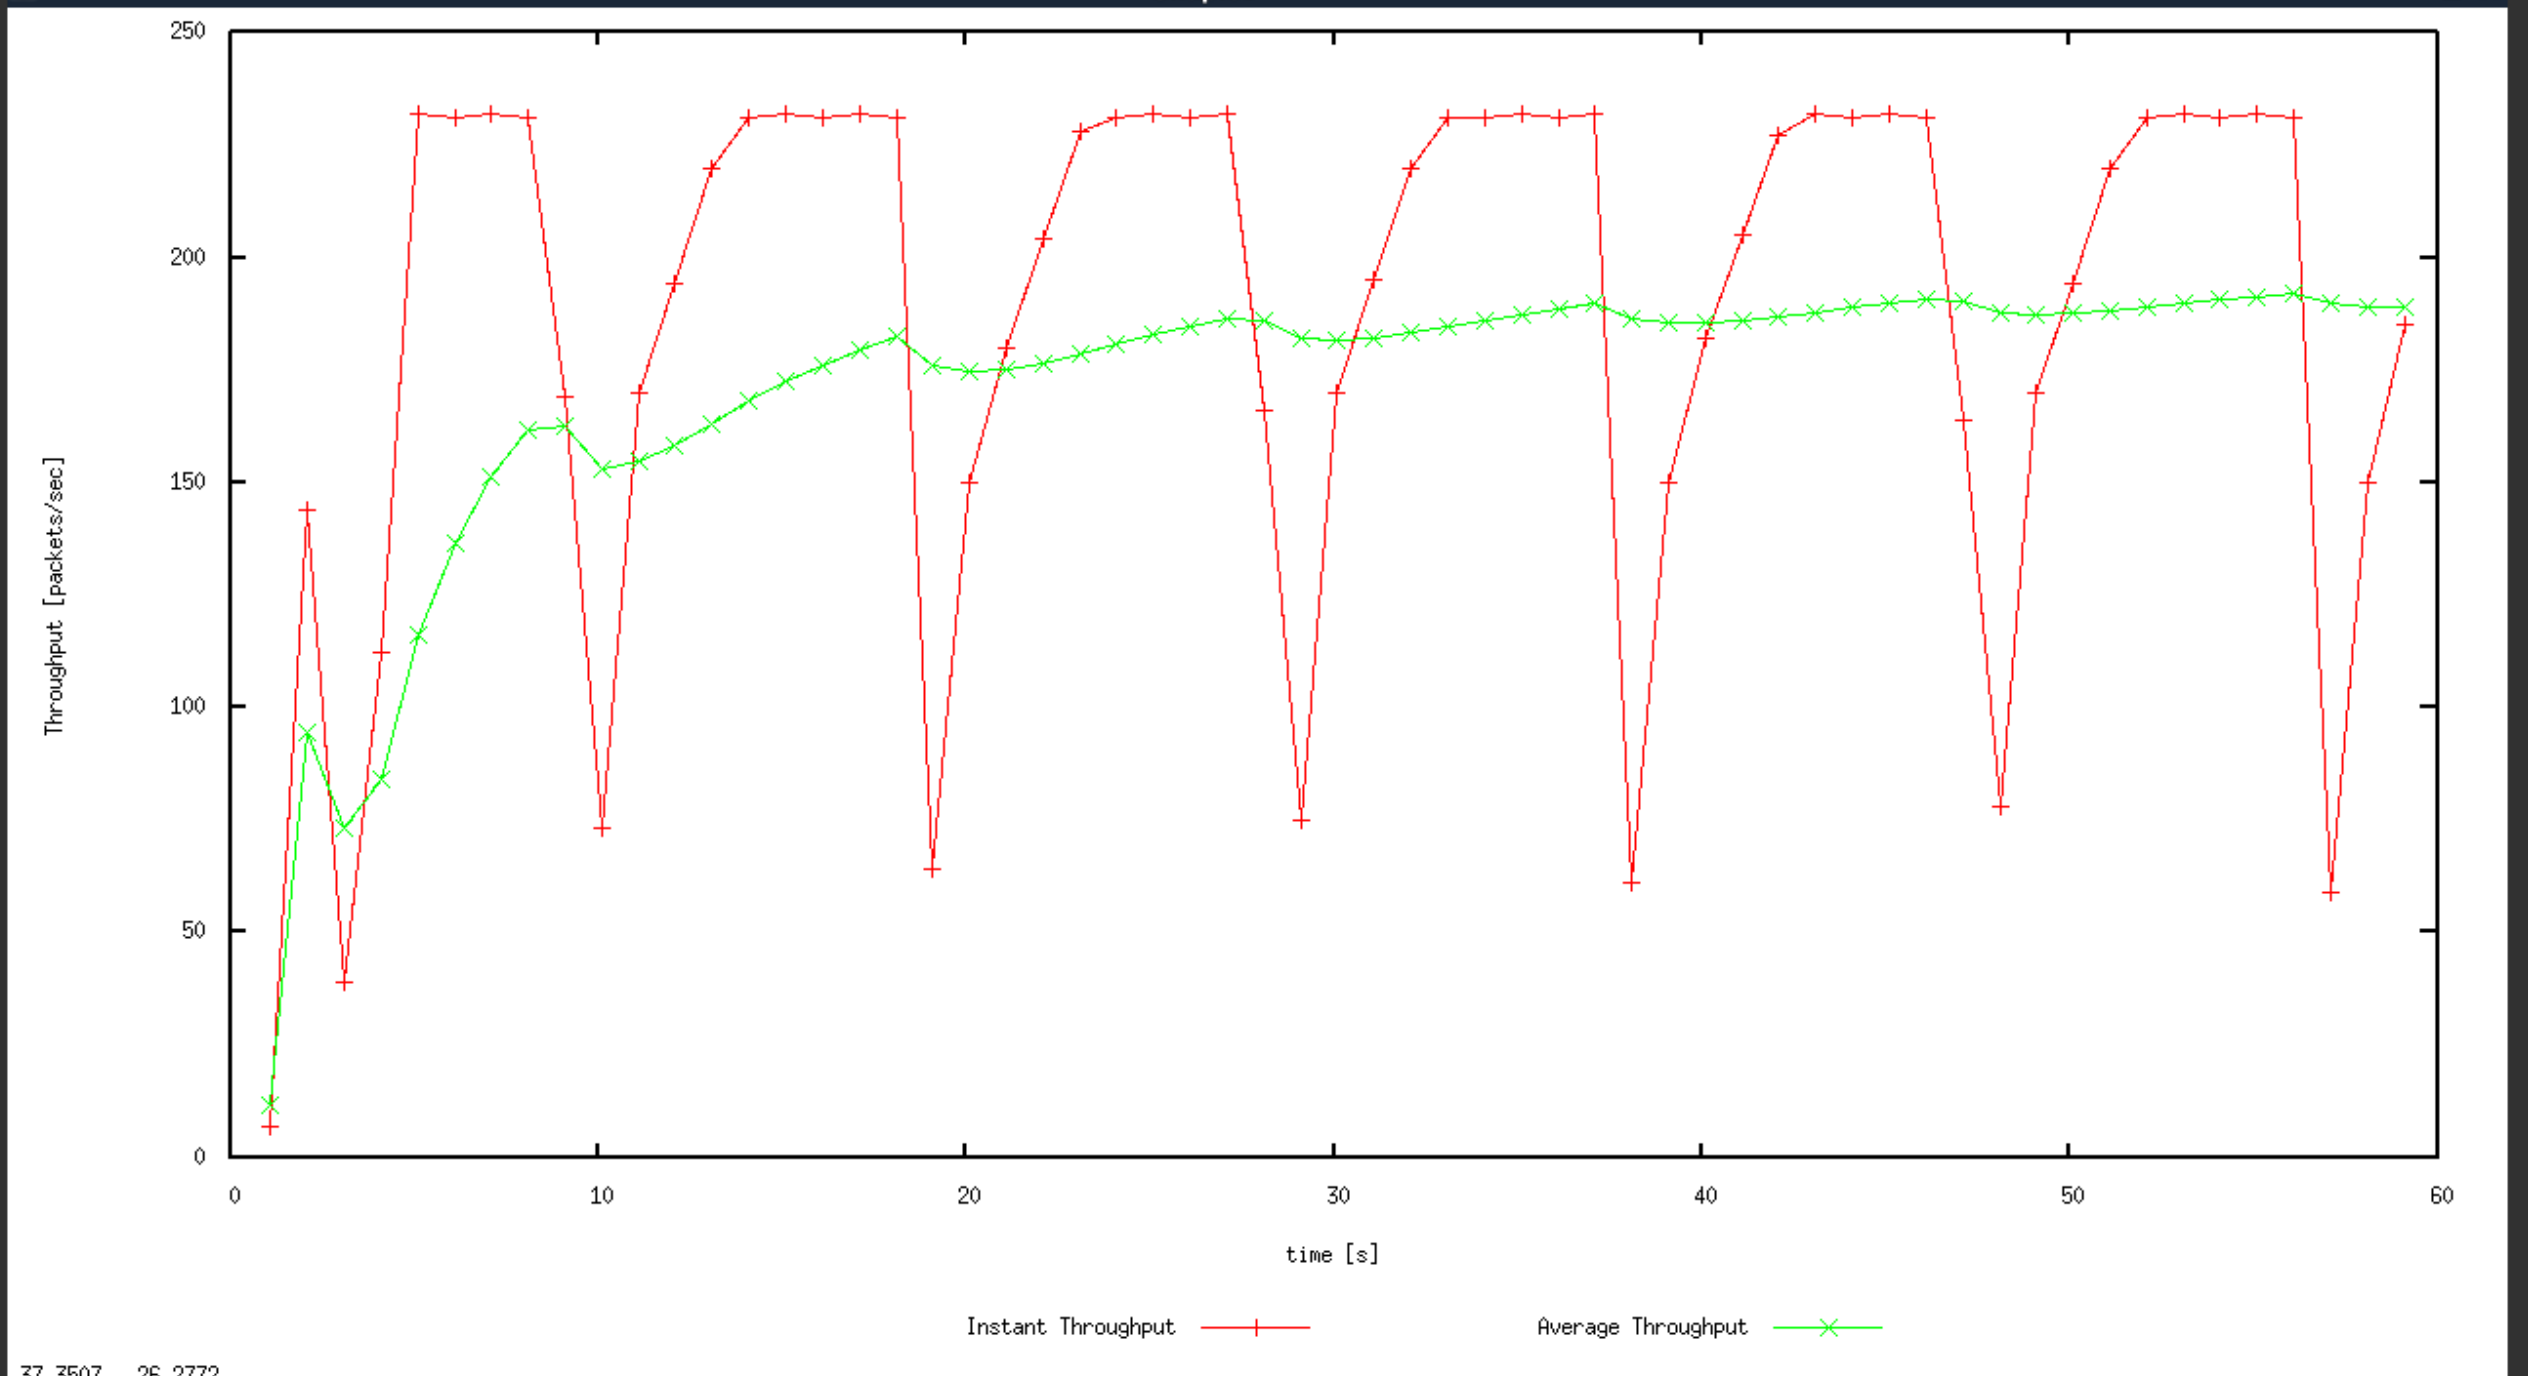
\includegraphics[width=\linewidth, height=0.43\textheight]{tt2f.png}
		\end{figure}
		\pagebreak
	\item 
		\begin{enumerate}
			\item Setting the maximum segment size to 66 gives no oscillation, that is, stable behaviour for the size of CWND. This is expected based on the answer to Q1.
			\item Average throughput in this case is 220.819 packets per second. Converting this to bits per second, we get 953938.08 bits per second. 
			\item This throughput is approximately 95.4\% of the link capacity.
		\end{enumerate}

	\item 
		\begin{enumerate}[label=\arabic*.]
			\item 
				\begin{enumerate}[label=(\alph*)]
					\item Maximum segment size is 67
					\item TCP Reno resets CWND to half the maximum value when CWND reaches 67.
					\item This is because the loss event was a triple duplicate ACK, and not a timout. TCP Reno resets CWND to half the maximum value on a triple duplicate ACK, unlike TCP Tahoe, which resets CWND to 0 on any loss event.
					\item TCP Reno does not transition back to slow start after a triple duplicate ACK loss event. This is becaues SSTHRESH is reset to half of the CWND size, which is also what CWND is reset to. Thus, in the next timestep, the CWND is not less than the SSTHRESH, they are actually the same. Therefore TCP Reno simply returns to AIMD.
				\end{enumerate}

				\begin{figure}[!htb]
					\centering
					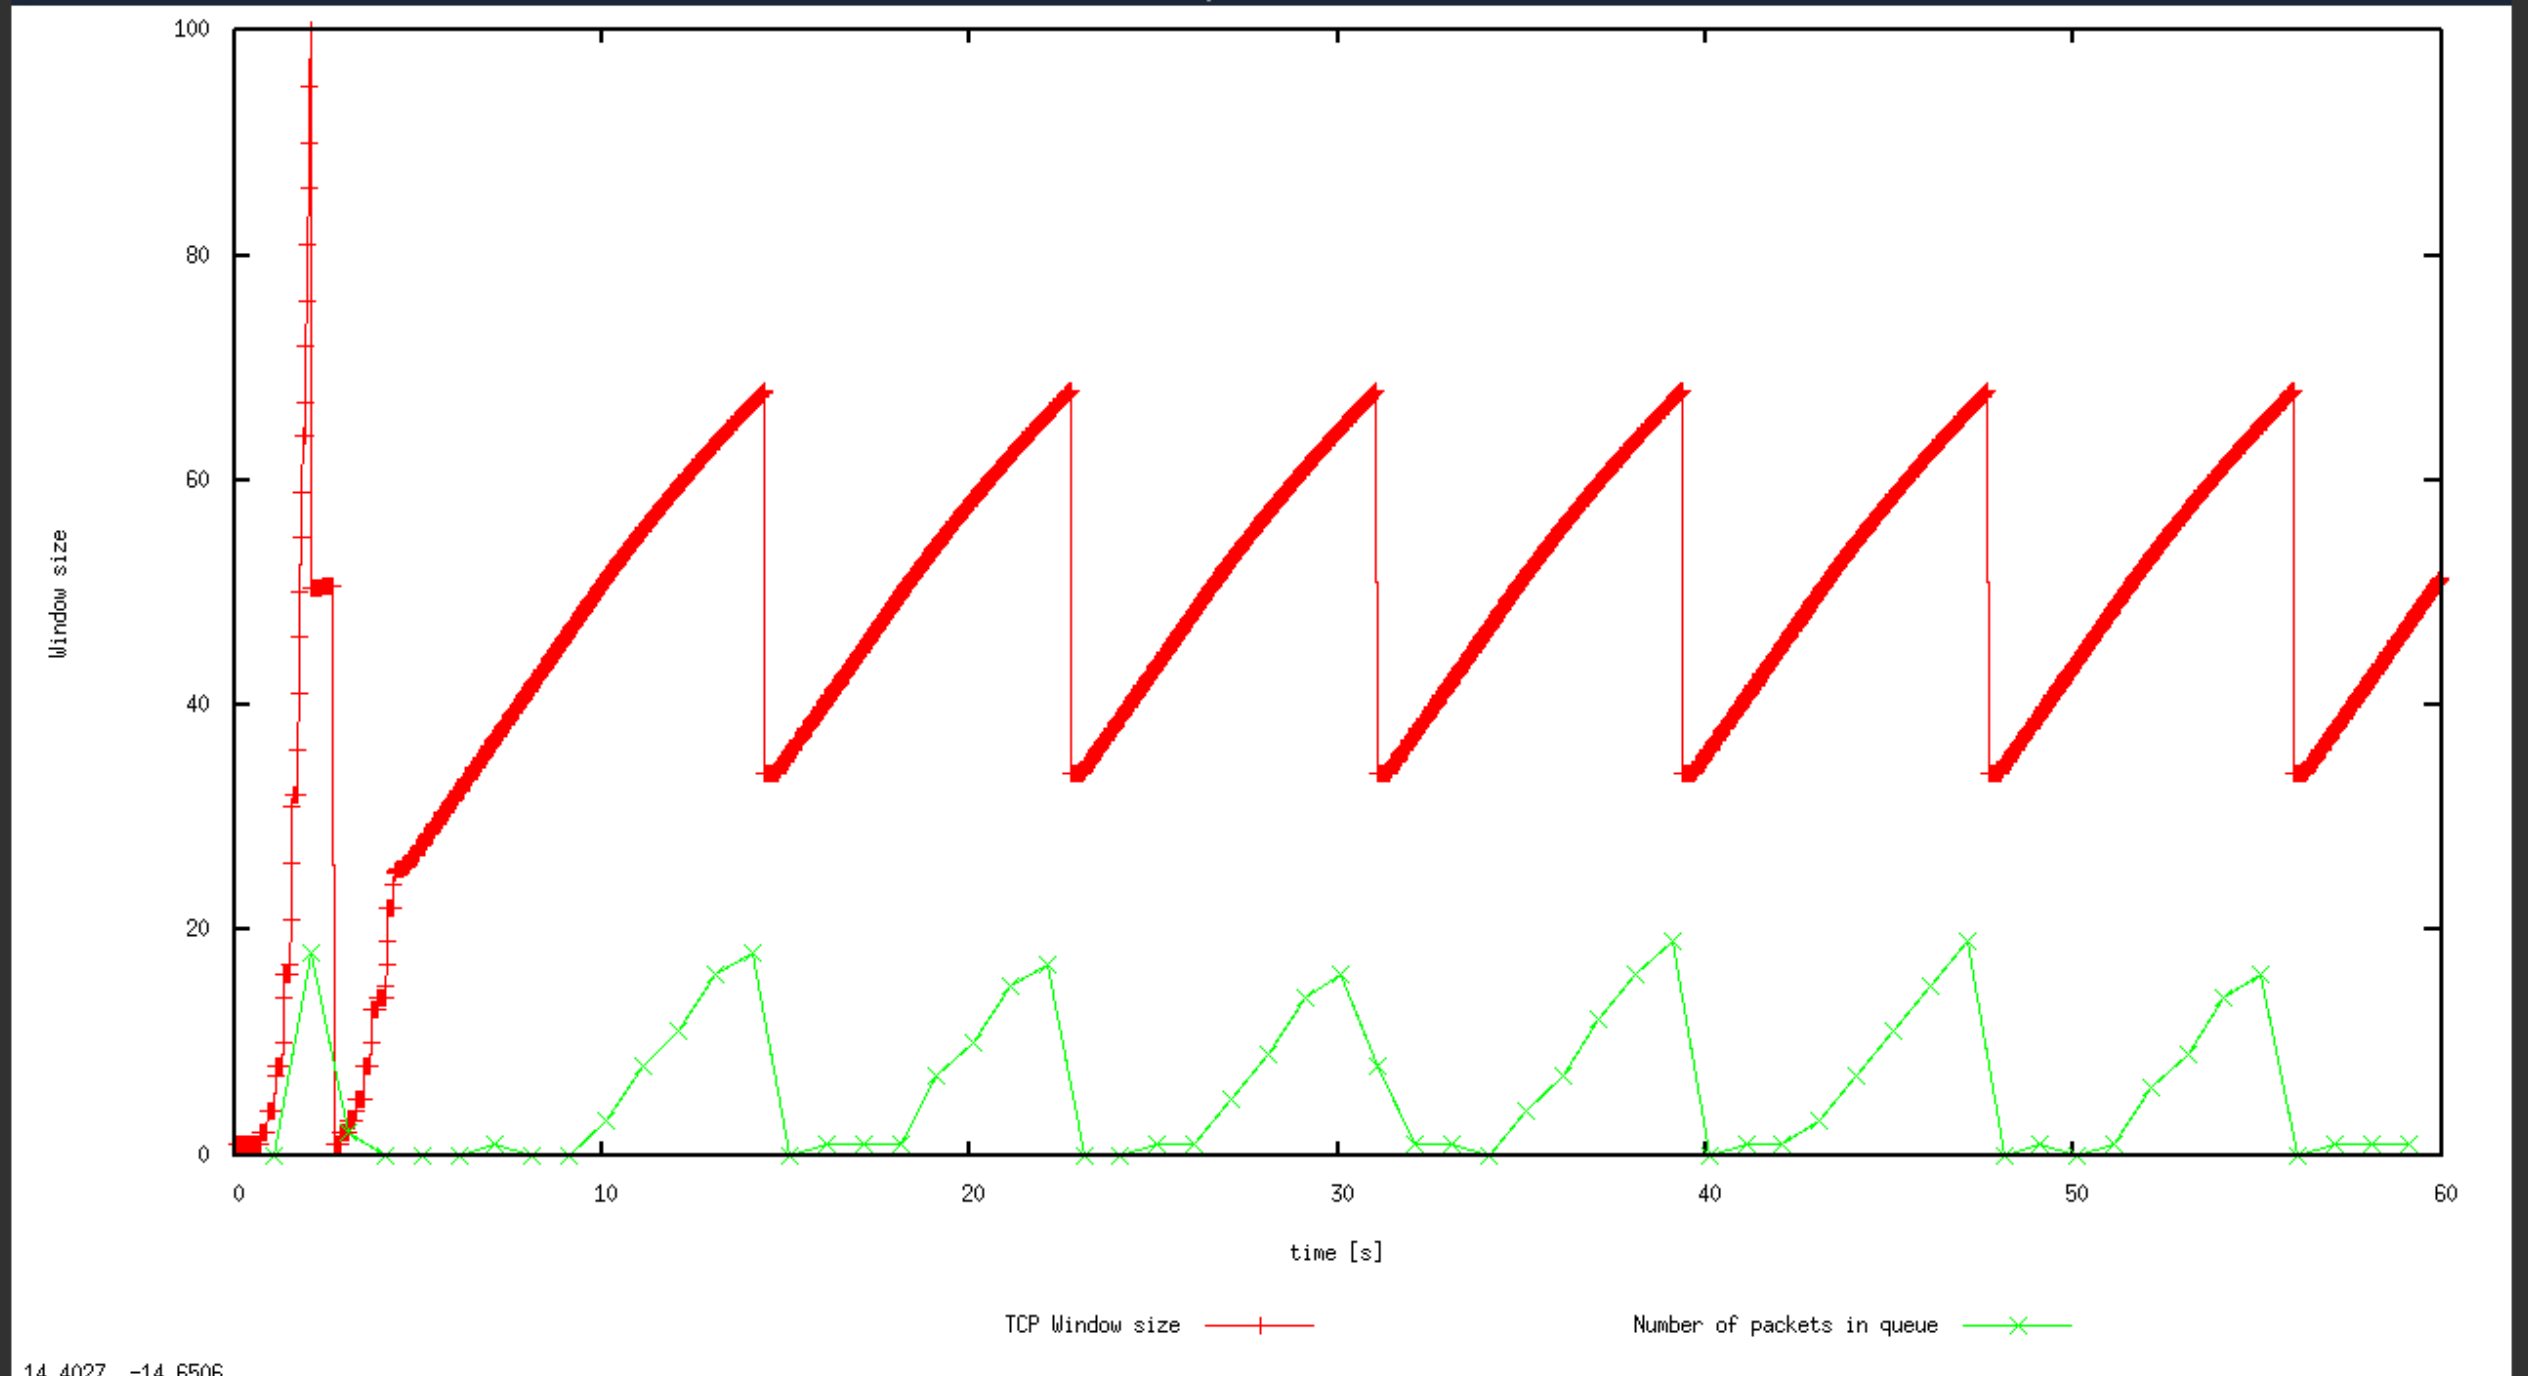
\includegraphics[width=\linewidth, height=0.43\textheight]{tr1f.png}
				\end{figure}
				\pagebreak

			\item Average throughput was 203.413 packets per second, which is 878744.16 bits per second. Clearly, TCP Reno has a higher average throughput.
				\begin{figure}[!htb]
					\centering
					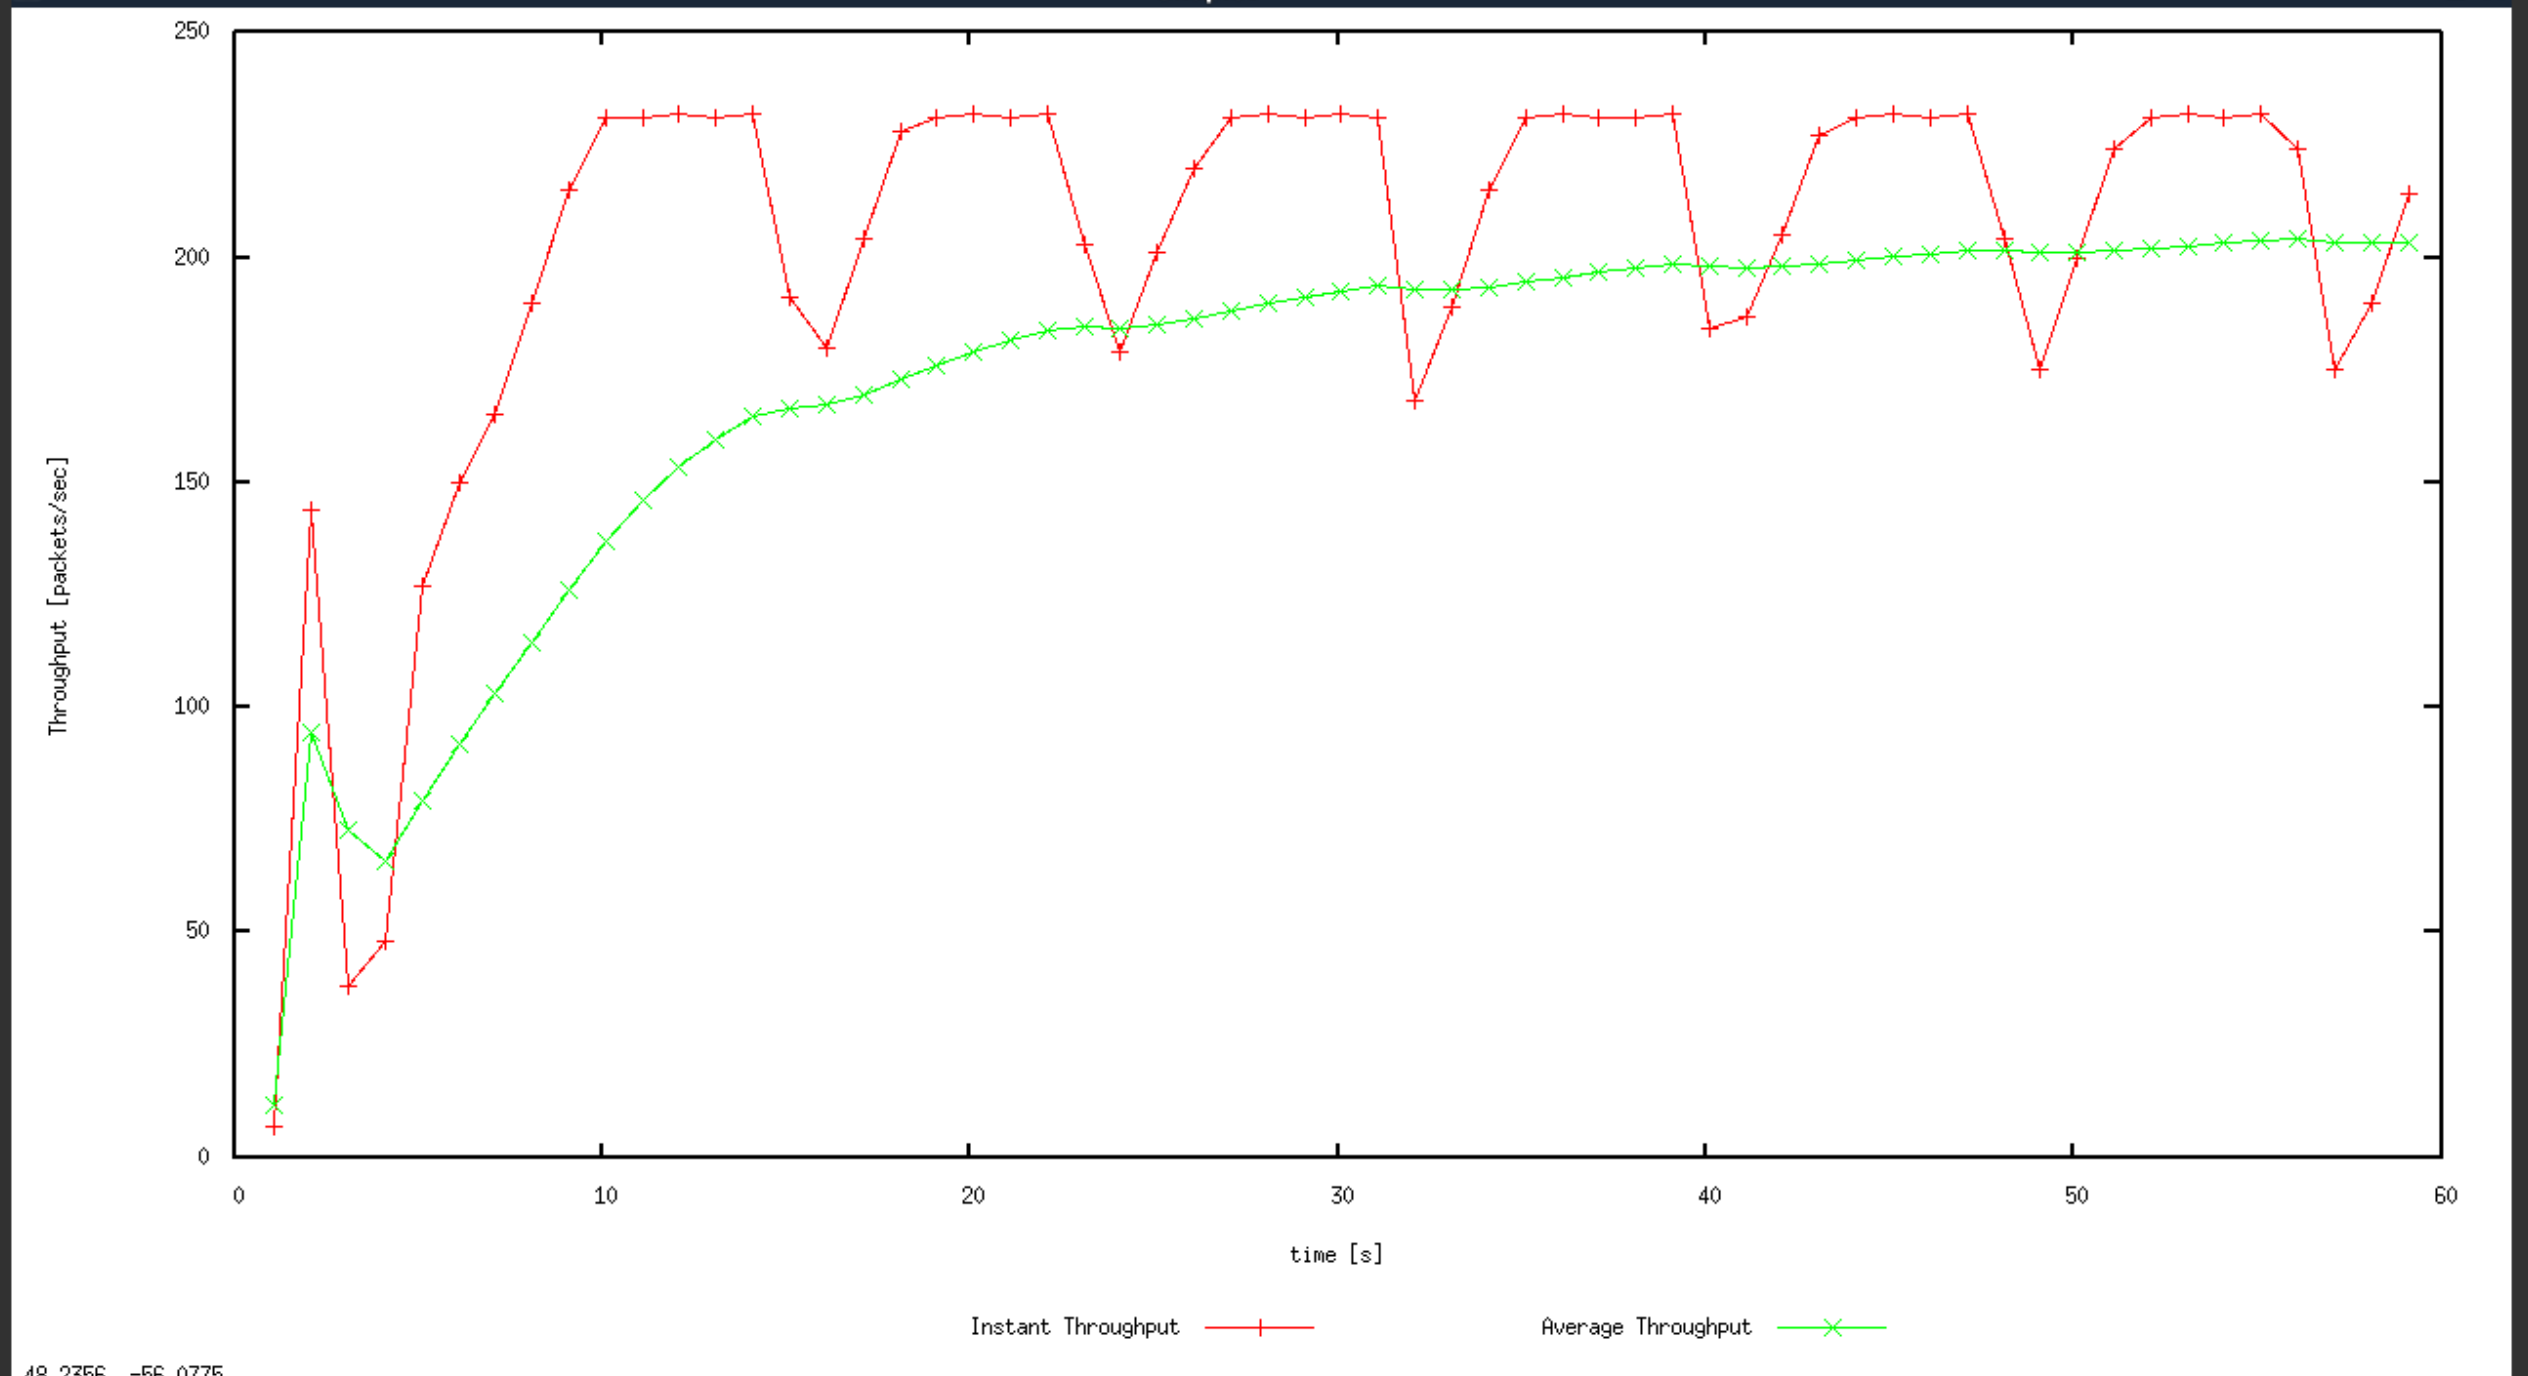
\includegraphics[width=\linewidth, height=0.43\textheight]{tr2f.png}
				\end{figure}
				\pagebreak
		\end{enumerate}
\end{enumerate}

\section{EXERCISE 3}
\begin{enumerate}[leftmargin=*]
	\item Initially all of the traffic will be from UDP, 4 Mbps, as the TCP connection is undergoing slow start. However, soon TCP will increase the sending window size, exponentially through the slow start probing. At some point, the TCP traffic will exceed 1 Mbps, and overflow the link, causing packet loss in both the UDP and TCP connections. As a result, TCP will reset the value of CWND to half of the value that the loss occurred at, as well as resetting SSTHRESH. TCP then transitions into AIMD immediately, as CWND is no longer less than SSTHRESH. TCP will now linearly increase its traffic, until overflow occurs again, and CWND is reset. The cycle will continue to repeat. The UDP traffic will sit around 4 Mbps, with inherent fluctuations, and TCP will oscillate up towards 1 Mbps, as CWND resets. UDP is clearly the red stream, and TCP the blue stream.
	\begin{figure}[!htb]
		\centering
		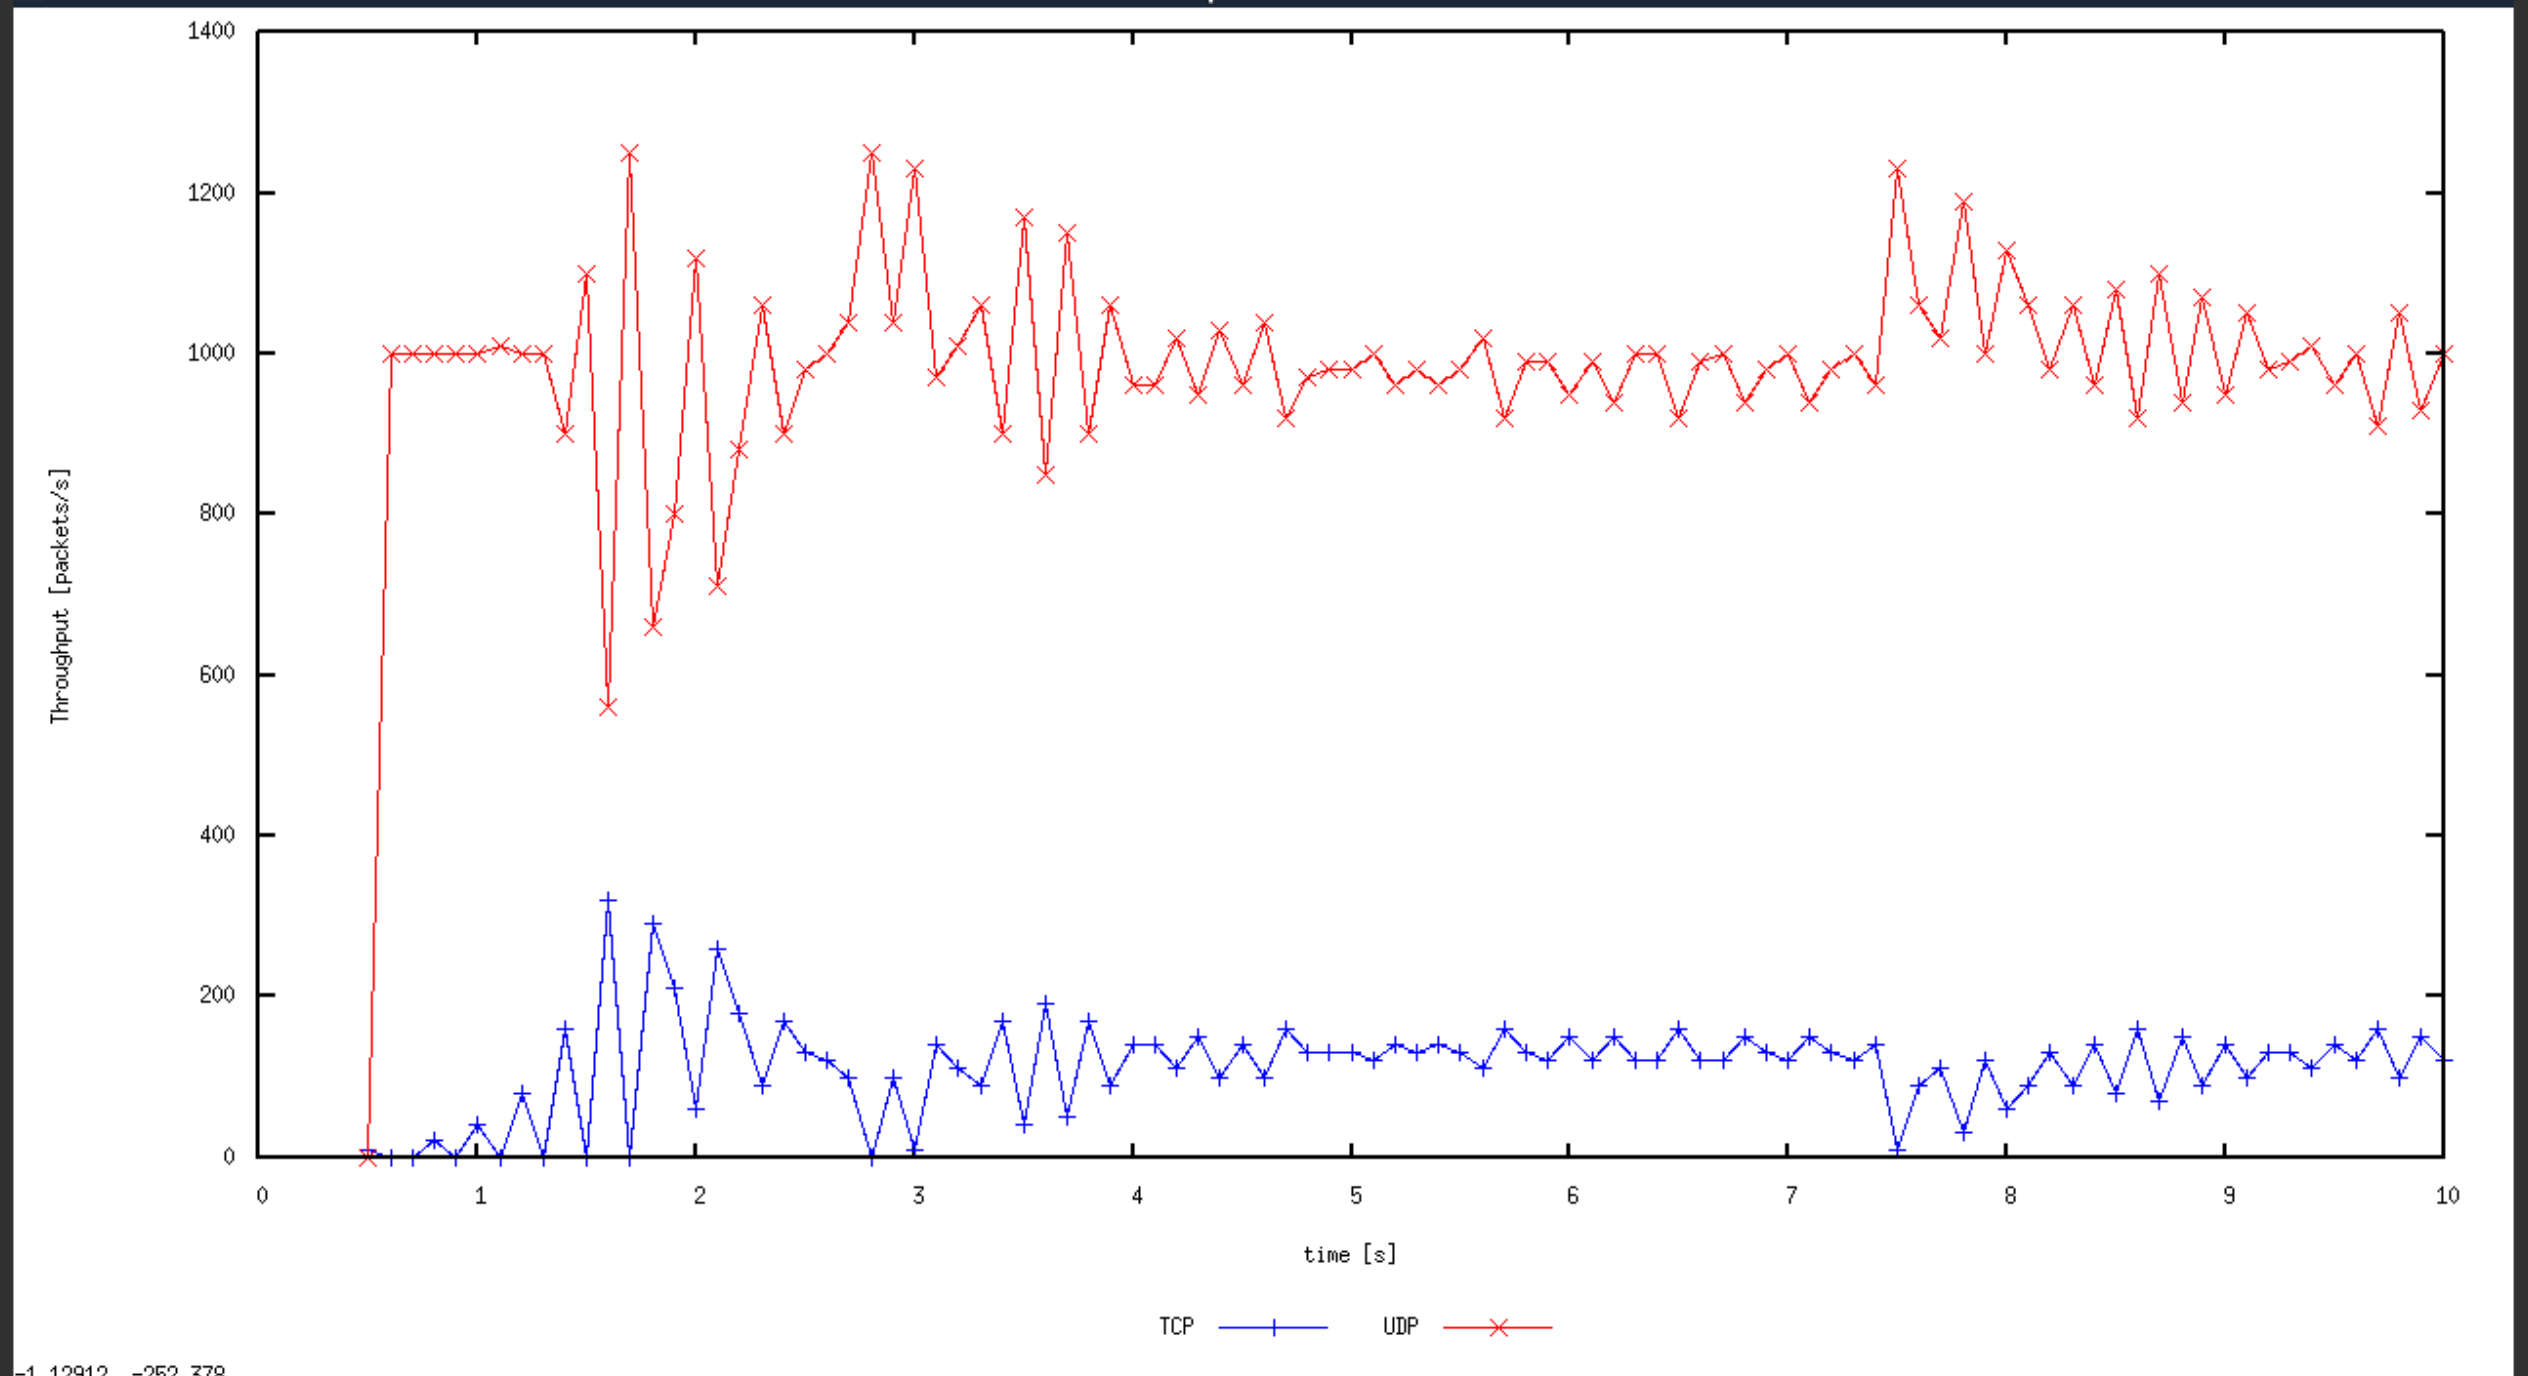
\includegraphics[width=\linewidth, height=0.43\textheight]{tu1f.png}
	\end{figure}
	
	\item UDP is transmitting at 4 Mbps upon launch of the program, as there is no regulation for UDP traffic. TCP intially has no throughput, as it is in the slow start phase, and is still beginning its growth. Eventually, the slow start increase will cause the first packet loss, and as such, CWND and SSTHRESH will both be reset. With TCP Reno, this puts an end to the slow start increase, as the loss events are all triple duplicate ACKs. Thus, TCP traffic incrementally increases under AIMD, so the TCP traffic will oscillate towards 1 Mbps, and begin to stabilise.
	\item UDP will always have the same throughput if the link has the capacity to support the full capacity of the UDP traffic. UDP will always send its full capacity through the link. In this sense, UDP is advantageous over TCP, as the transfer will be far faster. However, if everyone switched to UDP, with no congestion control mechanisms, the full capacity traffic of each UDP user will constantly overflow the link, causing packet loss. Packet loss will corrupt the file in file transfers, and would then require a retransmission, further burdening the link and causing more loss.
\end{enumerate}

\end{document}
